%
% IAT 267: Introduction to Technological Systems - A Course Overview
% Section: Sensors
%
% Author: Jeffrey Leung
%

\section{Sensors}
	\label{sec:sensors}
\subsection{Introduction}
	\label{subsec:sensors:introduction}
\begin{easylist}

	& \emph{Sensor:} Device which converts physical information into an electrical signals
	& May output variable resistance/voltage/capacitance/current

	& Types of sensors:
		&& \hyperref[subsec:technological-systems:categories]{Analog} sensors
			&&& Examples: Rotation, slider, temperature, touch, force, light
			&&& Often provides variable resistance
		&& \hyperref[subsec:technological-systems:categories]{Digital} sensors
		&& \emph{Passive sensor:} Sensor which requires its own power source to send a signal
		&& \emph{Active sensor:} Sensor which produces its own electrical signal through sensing
			&&& E.g. Piezoelectric, thermoelectric, or radioactive sensors

	& Physical design:
		&& \hyperref[subsec:electricity-and-circuit-design:types-of-electricity]{Piezoelectricity} can be used to measure force, flexure, acceleration, heat, acoustic vibrations (microphones)

\end{easylist}
\subsection{Characteristics to Sense}
	\label{subsec:sensors:characteristics-to-sense}
\subsubsection{Orientation}
	\label{subsubsec:sensors:characteristics-to-sense:orientation}
\begin{easylist}

	& \emph{Degree of freedom:} Axis along which an object is oriented
		&& E.g. In 3-d space, x/y/z are the 3 degrees of freedom
	& Rotation terminology:
		&& X-axis: Pitch/tilt
		&& Y-axis: Pan/yaw
		&& Z-axis: Roll

\end{easylist}
\subsubsection{Presence}
	\label{subsubsec:sensors:characteristics-to-sense:presence}
\begin{easylist}

	& Binary (present vs. not present)
	& Switches:
		&&& \emph{Foot switch:} Sensor which detects the binary presence of an object by contacting metal tape placed between foam spacers when pressure is applied
			&&&& Useful for small areas
		&&& \emph{Photoelectric switch:} Sensor which detects the binary presence of an object by detecting whether an object blocks the area between a light source and the sensor
		&&& \emph{Magnetic/reed switch:} Sensor which detects the binary presence of a magnetic field using two ferromagnetic contacts which connect in the presence of a magnetic object

\end{easylist}
\subsubsection{Position}
	\label{subsubsec:sensors:characteristics-to-sense:position}
\begin{easylist}

	& May be absolute or relative
	& \emph{Ranging sensor:} Sensor which detects the distance of an object relative to the sensor by sending a signal and comparing the energy reflected back to the original energy, or by detecting the time for the signal to reflect
		&& Constrained by distance, field of view, sweet-spot zones, and interference from other sensors
			&&& Solution: Constrain the environment (e.g. number of people, number of entrances or exits) rather than using more complex/numerous sensors
		&& \emph{Infrared distance sensor:} Sensor which detects the distance of an object relative to the signal by sending an infrared signal and calculating the amount of time for the signal to reflect back
			&&& Shorter ranges than ultrasonic sensors
		&& \emph{Ultrasonic sensor:} Sensor which detects the distance of an object relative to the signal by sending an ultrasonic signal and calculating the amount of time for the signal to reflect back
			&&& Longer ranges than infrared sensors
		&& E.g. Video tracking uses ranging sensors to automatically focus the camera lens
	& Multiple distance/presence sensors can determine the exact location of an object
		&& E.g. Multiple floor switches covering an area
		&& \emph{Trilateration:} Detection of the location of an object in a space by calculating distances from various points
			&&& Multiple signals at the same time may interfere with detection, so sensors must be alternated/cycled
	& A camera on a ceiling can track an object's position

\end{easylist}
\subsubsection{Motion and Video Tracking}
	\label{subsubsec:sensors:characteristics-to-sense:motion-and-video-tracking}
\begin{easylist}

	& Motion:
		&& \emph{Motion detector:} Sensor which detects changes in the infrared light in an area
		&& Velocity/acceleration can be calculated through sensing position over time

	& Video tracking:
		&& Cameras contain thousands of photocells which detect a wide range of light
			&&& Lighting conditions must be sufficient and consistent

\end{easylist}
\subsubsection{Identity}
	\label{subsubsec:sensors:characteristics-to-sense:identity}
\begin{easylist}

	& Camera/video detection of colour/images allows for shape/pattern recognition and tracking
		&& Advantages:
			&&& Adjustable distance to object
			&&& Detection of unique features
		&& Disadvantages:
			&&& Requires line of sight
			&&& Challenging to recognize objects from any angle and lighting

	& \emph{Barcode:} 1-d rectangle of white/black lines representing a unique binary code
		&& \emph{QR (Quick Response) code:} 2-d grid of white/black squares representing a unique binary code
		&& Advantages:
			&&& Can be read from variable angles
		&& Disadvantages:
			&&& Requires line of sight
			&&& Distortion from camera to digital recognition causes errors
			&&& Must be centred

	& \emph{Radio-frequency identification (RFID):} Tracking and identification of tags attached to objects which respond to radio signals
		&& RFID reader sends a short-range radio signal to an RFID tag, which returns a string of data
		&& \emph{Passive RFID system:} RFID system which includes a radio transceiver powered by induction from the received radio signal
			&&& Requires closer proximity and is cheaper than an active RFID system
		&& \emph{Active RFID system:} RFID system which includes a radio transceiver and a power supply
			&&& Has greater distance and is more expensive than an active RFID system
		&& Advantages:
			&&& Requires proximity rather than direct line of sight
		&& Disadvantages:
			&&& Short-ranged
			&&& May experience interference from radio noise

\end{easylist}
\subsection{Examples}
	\label{subsec:sensors:examples}
\begin{easylist}

	& Rotation sensor: Variable 3-pin sensor which outputs a resistance proportional to the rotation of the dial
		&& Functions similarly to a \hyperref[subsec:electricity-and-circuit-design:circuits]{potentiometer}
	& Slider sensor: Variable 3-pin sensor which outputs a resistance proportional to the distance from one side of the slider
		&& Functions similarly to a \hyperref[subsec:electricity-and-circuit-design:circuits]{potentiometer}
	& Temperature sensor: Sensor which outputs a voltage directly proportional to the temperature
		&& Formula:
		\begin{displaymath}
			T = \frac{v-200}{4}
		\end{displaymath}

		\begin{center}
			\Deactivate
			\begin{tabular}{ l r @{ = } l }
				where
				& $T$ & Temperature (\textdegree Celsius) \\
				& $v$ & Sensor value
			\end{tabular}
			\Activate
		\end{center}

		&& \emph{Thermal resistor:} Temperature sensor which changes resistance according to temperature
			&&& \emph{Resistance temperature detector (RTD):} Thermal resistor made from a naturally occurring material (e.g. copper, nickel, platinum) which changes resistance according to temperature
			&&& \emph{Thermistor:} Thermal resistor made from an artificial material (e.g. ceramic, polymer) which changes resistance according to temperature
				&&&& Resistance is inversely proportional to temperature
		&& \emph{Thermocouple:} Temperature sensor which utilizes a voltage difference at the connection of two conductors dependent on temperature
			&&& Created by Thomas Seeback
			&&& Commonly used
			&&& Cheap
			&&& Has standard connectors
			&&& Can measure a wide range of temperatures
				&&&& Can be inaccurate
			&&& E.g. A K-type thermocouple is made from the conductors nickel-chromium and nickel-aluminum
	& Capacitive sensor: Sensor which measures the amount of electrical charge
		&& Functions through glass
		&& Stored potential energy can be increased by using larger plates

	& Force sensor: Sensor which outputs a voltage directly proportional to the amount of force applied
		&& E.g. Placing a \hyperref[subsec:electricity-and-circuit-design:types-of-electricity]{piezoelectric} crystal between two metal plates and applying pressure to the plates will create voltage directly proportional to the amount of force

		&& Force-sensing resistor: Sensor which changes resistance according to the amount of force applied
			&&& Consists of a resistive material and a set of contacts; applying force to the sensor distorts the material allowing higher conductivity (see figure~\ref{fig:diagram-force-sensing-resistor})

			\begin{figure}[!htb]
				\centering
				\href
				{http://soundlab.cs.princeton.edu/learning/tutorials/sensors/node8.html}
				{
					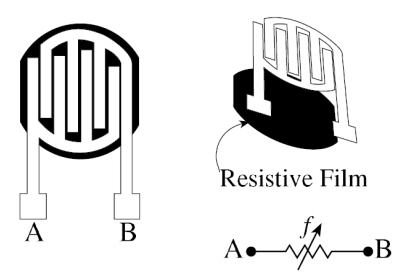
\includegraphics[scale=0.5]{force-sensing-resistor}
				}
				\caption{Diagram of a Force-Sensing Resistor}
				\label{fig:diagram-force-sensing-resistor}
			\end{figure}

		&& Flex sensor: Sensor which changes resistance according to the amount of distortion applied

		&& Pressure sensor: Sensor which measures the amount of pressure exerted by a fluid

		&& Methods to sense force:
			&&& Measurement of the acceleration of a known mass
			&&& Comparison of the unknown force against the gravitational force on the known mass (gravity-balance)
			&&& Conversion of the unknown force to a fluid pressure measured with a pressure transducer (pressure-sensing)

	& Photodetector/light sensor: Sensor which outputs a voltage proportional to the amount of light received
		&& \emph{Photodiode/quantum detector:} Light sensor which converts electromagnetic radiation into current in a semiconductor
			&&& Good detector of optical radiation
		&& \emph{Thermal detector:} Light sensor which absorbs infrared radiation and measures the \\ change in temperature

\end{easylist}
\subsection{Quality of Input}
	\label{subsec:sensors:quality-of-input}
\begin{easylist}

	& \emph{Transfer function:} Relationship/mapping of the electrical output signal by the physical input signal
		&& Calibration is done by applying known physical inputs and recording electrical outputs

	& \emph{Sensitivity:} Amount of change in output value given a change in input value
	& \emph{Accuracy:} Proximity of the measured value to the actual value
		&& Expressed as a percentage of the actual value

	& \emph{Precision:} Ability to create consistent output values within a given deviation from similar input values
	& \emph{Repeatability:} Ability to create consistent output values from a constant input value under the same environmental conditions
	& \emph{Stability:} Consistency of output values given a constant input value over a period of time
		&& Expressed as a percentage of the output
		&& Inverse of the amount of drift
		&& Reliable sensors have a drift of $< 2\%$

	& \emph{Range:} Difference between the minimum and maximum input limits/possibilities
		&& \emph{Span:} Difference between the minimum and maximum input values

	& \emph{Hysteresis:} Variation in output value for the same input value due to the change of the input value (i.e. increasing or decreasing)

	& \emph{Noise:} Fluctuations in the output values not caused by the input values
		&& May limit performance of a sensor

\end{easylist}
\clearpage
